%!TeX program = xelatex
\documentclass[numberedappendix,twocolumn,twocolappendix,apj]{openjournal}

\usepackage{latexsym}
\usepackage{graphicx}
\usepackage{amssymb}
\usepackage{longtable}
\usepackage{epsf}
\usepackage{amsmath}
\usepackage{graphicx}
%\DeclareMathOperator{\sech}{sech}
\usepackage{hyperref}
\hypersetup{colorlinks=true,linkcolor=blue,citecolor=blue,filecolor=blue,urlcolor=blue}
\usepackage{cleveref}
\usepackage{bm}
\usepackage{lipsum}
\usepackage{enumitem}
\usepackage{newtx}
\usepackage{gensymb}
\usepackage{booktabs}               % better table rules
\usepackage{multirow}
\usepackage{natbib}

%%%%%%%%%%%%%%%%%%%%%%%%%%%%%%%%%%%%%%%%%%%%%%%%%%
\usepackage[table]{xcolor}

\definecolor{hpurple}{HTML}{7E16DF}
\definecolor{hgreen}{HTML}{008F0F}
\definecolor{horange}{HTML}{FFA301}

\newcommand{\todo}[1]{\textcolor{hpurple}{\bfseries [todo: #1]}}
\newcommand{\addcite}{\textcolor{hpurple}{\bfseries [CITE]}}

\newcommand{\dd}{\rm d}
\newcommand{\eg}{\textit{e.g.}}
\newcommand{\ie}{\textit{i.e.}}
\newcommand{\panco}{\texttt{panco2}}
\newcommand{\bibtex}{\textsc{Bib}\!\TeX}

\newcommand{\refeq}[1]{eq.~(\ref{#1})}

\defcitealias{arnaud_universal_2010}{A10}
\newcommand{\aten}{\citetalias{arnaud_universal_2010}}


 %%%%%%%%%%%%%%%%%%%%%%%%%%%%%%%%%%%%%%%%%%%%%%%%%%
\begin{document}

\title{panco2: a Python library to measure intracluster medium pressure profiles from Sunyaev-Zeldovich observations}
\shorttitle{\panco: pressure profiles from tSZ maps}

\author{F. K\'eruzor\'e$^{1,2,\star}$}
\author{F. Mayet$^{2}$}
\author{E. Artis$^{2}$}
\author{L. E. Bleem$^{1}$}
\author{J.-F. Mac\'ias-P\'erez$^{2}$}
\author{M. Mu\~noz-Echeverr\'ia$^{2}$}
\author{L. Perotto$^{2}$}
\author{F. Ruppin$^{3}$}
\author{others?}

\affiliation{
    $^1$High Energy Physics Division, Argonne National Laboratory, 9700 South Cass Avenue, Lemont, IL 60439, USA \\
    $^2$Univ. Grenoble Alpes, CNRS, Grenoble INP, LPSC-IN2P3, 53, avenue des Martyrs, 38000 Grenoble, France \\
    $^3$Univ. Lyon, Univ. Claude Bernard Lyon 1, CNRS/IN2P3, IP2I Lyon, F-69622, Villeurbanne, France
}
\thanks{$^{\star}$E-mail:fkeruzore@anl.gov}

\shortauthors{K\'eruzor\'e et al.}

%%%%%%%%%%%%%%%%%%%%%%%%%%%%%%%%%%%%%%%%%%%%%%%%%%%%%%%%%

\begin{abstract}
    We present \panco, an open-source \texttt{Python} library designed to fit pressure profiles in Sunyaev-Zeldovich maps.
    The fitting procedure is based on forward modeling of the total observed signal, allowing to take into account usual features of millimeter observations, such as beam smearing, data processing filtering, and point source contamination.
    \panco\ offers a large flexibility in the inputs that can be handled and the analysis options, enabling refined analyses and studies of systematic effects.
    We detail the functionalities of the code, the algorithm used to infer pressure profile measurements, and the typical data products.
    We present examples of running sequences, and the validation on simulated inputs.
    The code is available on \href{https://github.com/fkeruzore/panco2}{github}, and comes with an extensive technical documentation to complement this paper.
\end{abstract}

\keywords{Cosmology: large-scale structure of Universe}

\maketitle

\vspace{1cm}

\twocolumngrid

%%%%%%%%%%%%%%%%%%%%%%%%%%%%%%%%%%%%%%%%%%%%%%%%%%
%%%%%%%%%%%%%%%%% BODY OF PAPER %%%%%%%%%%%%%%%%%%

\section{Introduction}
\label{sec:intro}

%%% Why clusters are cool
Galaxy clusters are deeply interesting physical objects.
Their abundance in mass and redshift is tightly linked to cosmic evolution, and can therefore be used as a cosmological probe \citep[see \eg][for a review]{allen_cosmological_2011}.
In order to exploit this property, large sky surveys have been used to build catalogs of serendipitously detected clusters at different wavelengths, such as X-rays \citep[\eg][]{liu_erosita_2022}, optical \citep[\eg][]{des_collaboration_dark_2020}, and millimeter-waves \citep[\eg][]{bleem_sptpol_2020}.

%%% Why SZ clusters are the coolest
Among these, one of the wavelengths of choice for the detection of galaxy clusters is the millimeter domain.
Clusters can be observed at such frequencies through the Sunyaev-Zeldovich effect \citep[SZ,][]{sunyaev_observations_1972}, \ie\ the spectral distortion of the cosmic microwave background (CMB) due to the Compton scattering of its photons on the free electrons of gas along the line of sight.
The SZ effect is often separated in different components, depending on the origin of the energy transferred from the electrons; the main components being, by order of decreasing importance, the thermal (tSZ) and kinetic \citep[kSZ,][]{sunyaev_velocity_1980} effects \citep[see][for a recent review of the SZ effects]{mroczkowski_astrophysics_2019}.
Catalogs of clusters detected through their tSZ signal are particularly interesting for cosmological applications, as the amplitude of the tSZ effect does not suffer from cosmological dimming \citep{carlstrom_cosmology_2002}.
As a result, modern millimeter-wave sky surveys have brought us some of the largest and deepest cluster samples to date, with the catalogs built from the Atacama Cosmology Telescope \citep[ACT,][]{hilton_atacama_2021}, the South Pole Telescope \citep[SPT,][]{bleem_sptpol_2020}, and \textit{Planck} \citep{planck_collaboration_planck_2016-2} surveys.

%%% Why do we measure pressure profiles
% tSZ depends on ICM pressure, therefore knowing pressure we know what to look for
The amplitude of the tSZ distortion is directly proportional to the electron pressure in the gaseous intracluster medium (ICM) integrated along the line of sight.
This link between tSZ signal and ICM pressure motivates studies of the pressure distribution in the ICM -- in its simplest form, as a spherically symmetric pressure profile.
For example, matched-filtering cluster detection algorithms may require a prior assumption on the overall shape of the ICM pressure profile \citep[\eg][]{melin_comparison_2012}, in which case a poor knowledge of this property of clusters may lead to a poorly constructed cluster sample.
Similarly, the power spectrum of the tSZ effect on the sky, which can be used to constrain cosmology, strongly relies on an assumption of the pressure profile of clusters, and the recovering of cosmological parameters can be severely affected by its poor knowledge \citep{ruppin_impact_2019}.
% Early studies told us they should all be the same
The mean pressure profile of galaxy clusters has been investigated using different cluster samples over the last decade.
Early works conducted on local, X-ray selected samples, such as \citet[][hereafter \aten]{arnaud_universal_2010}, converged towards a ``universal'' pressure profile, undergoing self-similar redshift and mass evolution \citep[see also \eg][]{battaglia_cluster_2012-1, planck_collaboration_planck_2013}
In these studies, the main determining factor for the shape of the pressure profile of a cluster was its dynamical state, with relaxed clusters exhibiting a steeper pressure profile in their core.
% But hey that was wrong because feedback and stuff
% We'd do simulations but their subgrids need us so the snake is eating its own tail

\textcolor{lightgray}{\lipsum[1]}

%%% How do we measure pressure profiles
% Can be from Xrays
% But that works better for low-z and high-M thingies
% Can be from SZ
% Need to resolve them but can be done

%%% What is this paper
% In this work we present a software to go from SZ map to P(r)
An earlier version of \panco\ was described in \citet{keruzore_panco2_2021}, which offered less flexibility in the analysis, as the only data that could be analyzed was maps from the NIKA2 camera 150~GHz channel\citep{adam_nika2_2018, perotto_calibration_2020}.
This software has already been used for different studies based on NIKA2 data \citep[\eg][]{artis_psz2_2022,munoz-echeverria_multi-probe_2022,munoz-echeverria_lpsz-clash_2022}.
Here, we present a generalization of the code, that makes it able to perform pressure profile extractions from arbitrary data formats.



\textcolor{lightgray}{\lipsum[2]}


% ========================================================================== %
\section{Algorithm} \label{sec:algo}

The goal of \panco\ is to infer a measurement of a pressure profile and of its confidence intervals from the SZ map of a cluster.
The overall workflow implemented in \panco\ to perform this measurement is presented in Figure~\ref{fig:workflow}.
It is based on the forward modeling of the SZ map and on Monte-Carlo Markov Chain (MCMC) sampling of the probability distribution for the pressure profile parameters given the input data.
In this section, we detail each step of the analysis, as well as the inputs to be given to \panco\ and the results it produces.

\begin{figure*}[htp]
    \centering
    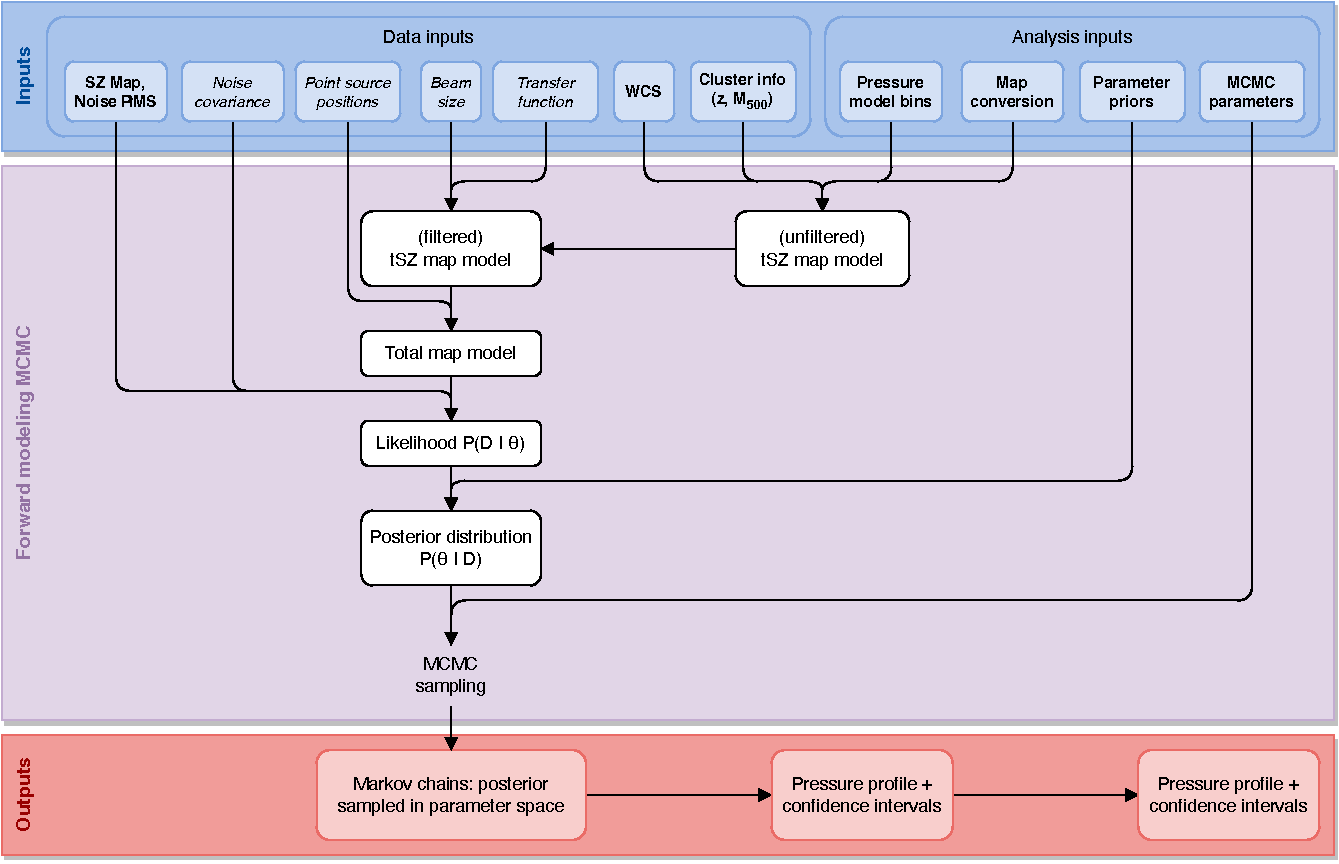
\includegraphics[width=.9\linewidth]{Figures/workflow.drawio.pdf}
    \caption{
        Schematic workflow of the \panco\ algorithm, from its inputs (blue), to the forward modeling and MCMC sampling (purple), and results (red).
        Required and optional inputs are denoted with boldface and italic fonts, respectively.
    }
    \label{fig:workflow}
\end{figure*}

% -------------------------------------------------------------------------- %
\subsection{Data inputs} \label{sec:algo:inputs}

The main input of \panco\ is a mapping of a patch of the sky containing SZ signal.
The code uses the FITS standard \citep{wells_fits_1981} to correctly map sky coordinates to pixels using the flat-sky approximation.
The map to be fitted must therefore be contained within a FITS file, that must include the following ingredients:

\begin{itemize}[leftmargin=*]
    \item An extension in which the data is the SZ map to be fitted, and the header includes the World Coordinate System (WCS) used to create the map;
    \item An extension in which the data represent an estimate of the expected root mean squared (RMS) error for each pixel of the data map.
\end{itemize}

Such a file constitutes the minimum data input for \panco\ to proceed fitting a pressure profile.
Using these inputs, the user may choose to only use a square portion of the map, by specifying the sky coordinates of its center and its side.

Additional inputs can be provided to account for various data features.
\paragraph{Beam smearing} the user may provide the width of a Gaussian function to account for point spread function (PSF, hereafter referred to as ``beam'') filtering (see \S\ref{sec:algo:fwdmod});
\paragraph{Transfer function} Fourier filtering due to data processing and/or scanning strategy can be accounted for in the analysis (see \S\ref{sec:algo:fwdmod});
\paragraph{Point source contamination} the position on the sky of point sources, as well as their fluxes and uncertainties, can be used to account for the contamination and marginalize over its amplitude (see \S\ref{sec:algo:fwdmod});
\paragraph{Correlated noise} the covariance matrix between the noise of pixels in the map can be provided (see \S\ref{sec:algo:likelihood}).

% -------------------------------------------------------------------------- %
\subsection{Pressure profile model} \label{sec:algo:press}

The electron pressure distribution in the ICM is modeled in \panco\ as a radial pressure profile, implying spherical symmetry of the ICM.
The most widely used parametrization for ICM pressure profiles, called the generalized Navarro-Frenk-White model \citep[gNFW,][]{zhao_analytical_1996, nagai_effects_2007}, is known to have several shortcomings.
In particular, the very self-constrained shape of the functional form of the profile and the important correlations in the parameter space make model fitting complex, and the recovered parameter values hard to interpret \citep[see \eg][]{nagai_effects_2007, battaglia_cluster_2012-1, sayers_evolution_2022}.

In order to try to circumvent these issues, \panco\ uses a more flexible parametrization of the pressure profile, in which the pressure distribution is modeled as a power law evolution in concentric spherical shells.
In this modeling\footnote{Several papers in the literature have dubbed this modeling a ``non-parametric'' approach; as this is not strictly true, since the model is parametric, we will refrain from using this term, and refer to our model as ``radially binned''.}, the model parameters are the values $P_i$ of the pressure profile at predefined radii from the cluster center $R_i$, with a power law interpolation between the radii:
\begin{equation}
    \label{eq:algo:pressure_profile}
    P(r \in [R_i, R_{i+1}[) = P_i \left(r / R_i\right)^{-\alpha_i},
\end{equation}
where $\alpha_i = - \log(P_{i+1} / P_i) / \log(R_{i+1} / R_i)$. \\
Outside of the radial bins, the pressure profile is extrapolated using the power-law evolution of the first (last) bin.
In addition to being more flexible and having generally lesser correlations in the parameter space, this parametrization can be integrated along a line of sight analytically through Abell transform, by following \eg\ \citet{romero_multi-instrument_2018}.

The main downside to this pressure profile modeling lies in the need to specify the radii $R_i$ used in \refeq{eq:algo:pressure_profile} \textit{a priori} when performing a fit.
There is no obvious, fail-safe way to define this radial binning.
A user may choose a binning motivated by the data coverage (\eg\ with radii that, projected on the sky plane, are separated the beam of the instrument used to build the map); but looking at the same data, another user may be motivated by sample studies over several cluster, and wish to define a binning in units of a characteristic radius of the cluster (\eg\ $R_{500}$).
As a result, model dependence may arise in the results produced by \panco.
This point will be addressed \todo{later}.

% -------------------------------------------------------------------------- %
\subsection{Forward modeling: from pressure profile to SZ map} \label{sec:algo:fwdmod}

The approach used by \panco\ to fit pressure profiles on SZ maps is forward modeling.
In that framework, a pressure profile model -- determined by \refeq{eq:algo:pressure_profile} -- is used to generate a map that can be compared to data.
This approach has been vastly used in the estimation of pressure profiles from tSZ maps, especially in the context of resolved follow-up of galaxy clusters with \eg\ NIKA2 \citep[\eg][]{munoz-echeverria_multi-probe_2022,keruzore_exploiting_2020}, MUSTANG(2) \citep[\eg][]{romero_galaxy_2017,romero_pressure_2020}, Bolocam \citep[\eg][]{sayers_evolution_2022}, or ALMA \citep[\eg][]{di_mascolo_joint_2019}.
This section details the different steps used in that process.

\paragraph{Line of sight integration}

The amplitude of the tSZ effect in a direction $\theta$ on the sky is named the Compton parameter $y$, and is proportional to the integral along of the electron pressure along the line of sight (LoS):
\begin{equation}
    \label{eq:algo_ysz}
    y(\theta) = \frac{\sigma_\textsc{t}}{m_{\rm e}c^2} \int_{\rm LoS(\theta)} P_{\rm e} \; \dd l,
\end{equation}
where $\sigma_\textsc{t}$ is the Thompson cross-section, and $m_{\rm e} c^2$ is the electron resting energy. \\
In \panco, we perform this integration analytically, by following the derivation presented in Appendix A of \citet{romero_multi-instrument_2018}, using the spherically symmetric case (in the notation of \citeauthor{romero_multi-instrument_2018}, $a_i = b_i = c_i = 1 \; \forall \; i$).
This allows us, for any given pressure profile, to create a Compton parameter map in the same coordinate system as the data, \ie\ an estimate of the value of $y$ for each pixel in the map.

\paragraph{Conversion}

Depending on the data product available, and on the convention used in the raw data processing software employed to create these data products, tSZ maps can have a variety of units (\eg\ surface brightness, CMB temperature fluctuation).
These units can usually be converted to Compton$-y$ through a scalar conversion coefficient, $C_{\rm conv}$, which can depend on many different quantities that may be difficult to estimate, or even fluctuate during observations, such as instrumental bandpasses, weather conditions, instrumental calibration, or even temperature of the ICM through relativistic corrections to the tSZ effect \citep{mroczkowski_astrophysics_2019}.
As a result, the conversion coefficient is affected by an uncertainty.
In \panco, this coefficient is treated as a parameter in the model, for which a prior distribution needs to be specified (see \S\ref{sec:algo:mcmc}), allowing to propagate the uncertainty on the conversion of the map to the pressure profile estimate.
This means that a vector in the parameter space will contain a value of a conversion coefficient, which \panco\ multiplies the model $y-$map by to get a map in the same units as the input data.
In case the input data is already in units of Compton$-y$, this coefficient may still be used to propagate multiplicative calibration uncertainty by centering the prior distribution on 1.
\todo{zero level}

\paragraph{Filtering}

The tSZ maps constructed by any instrument are affected by different types of filtering.
The instrumental PSF acts as a filter that smooths the data by suppressing signal at small scales.
In its forward modeling approach, \panco\ is able to take into account this filtering by convolving the model $y-$map with a 2D Gaussian filter, the width of which can be specified by the user.

In addition, during the data reduction process used to create tSZ maps from raw data, filtering can occur, often suppressing signal at large angular scales.
This filtering is usually accounted for through a transfer function, quantifying the signal filtering in the Fourier space, and evaluated during the data processing.
\panco\ can account for this effect by filtering the map with a transfer function provided by the user.
Two different types of transfer functions can be provided:
\begin{itemize}[leftmargin=*]
    \item a 1D transfer function: assuming that the filtering is isotropic, \panco\ can convolve model maps with a 1D kernel specified by the user as angular frequencies $k$ and their associated filtering ${\rm TF}(k)$;
    \item a 2D transfer function: if the filtering on the sky cannot be assumed to be isotropic, the user may specify 2D angular scales $(k_x, k_y)$ and their corresponding filter ${\rm TF}(k_x, k_y)$.
\end{itemize}
A thorough discussion of the impact of choosing a 1D or 2D transfer function -- in the case of NIKA2 data, in which the filtering is mildly anisotropic -- can be found in \citet{munoz-echeverria_multi-probe_2022}.

\paragraph{Point source contamination}

After applying the different filters, the \panco\ model map is a map of the tSZ signal, in the unit and mapping as the input data, and having been affected by the same signal filtering.
It is therefore comparable to the tSZ signal in the input map.
But millimeter-wave maps of cluster regions may also include astrophysical signal from other sources.
In particular, signal from millimeter-emitting galaxies can often be found in such maps.
These galaxies can be foreground, background, or cluster members, and their emission can be thermal (in the case of dusty star-forming galaxies), or synchrotron (for radio-loud AGN).
In any case, this signal manifests as a contamination for tSZ science, and must be accounted for in data analysis, lest the recovered pressure profile be biased.

In its forward modeling approach, \panco\ uses the methodology described in \eg\ \citet{keruzore_exploiting_2020}, in which point source models may be added to the tSZ model map in order to model the total signal in the map.
The spatial model of each source is given by the instrumental PSF, and their fluxes are treated as model parameters, with priors specified by the user (see \todo{later}).
If the flux of a source is well known from external data, this prior will be tight, and serve as a propagation of its uncertainty to the recovered pressure profile.
Otherwise, if a source is known to be present but little is known about its flux, large priors can be used, in which case \panco\ will constrain the sum of the tSZ signal and the point source flux\footnote{\panco\ is able to constrain the sum of the two because of the different spatial distribution of the tSZ and point source fluxes.}.
To account for point source contamination in the analysis, the user must therefore provide \panco\ with a position (in sky coordinates) and a probability distribution for the flux (in input map units) for each of the sources considered.

% -------------------------------------------------------------------------- %
\subsection{Likelihood} \label{sec:algo:likelihood}

The process described in \S\ref{sec:algo:fwdmod} allows \panco\ to compute a model map that is comparable to the input data from any position in the parameter space.
To summarize, a vector in this parameter space, $\vartheta$, has the following components:
\begin{itemize}[leftmargin=*]
    \item $P_0, \dots P_n$: the value of the pressure profile at each predefined radius $R_0, \dots R_n$ ; \\
    \item $C_{\rm conv}$: the conversion coefficient from Compton$-y$ to input map units;
    \item $Z$: a zero-level for the map;
    \item If provided, $F_0, \dots F_m$: the fluxes of point sources in the map, in input map units.
\end{itemize}

The comparison between the model map and the input data is performed through a Gaussian likelihood function:
\begin{align}
    \nonumber -2 \log \mathcal{L}(\vartheta) & \equiv -2 \log P(D | \vartheta) + {\rm cst.} \\
        & = \left[D - M(\vartheta)\right]^{\rm T} \mathbf{C}^{-1} \left[D - M(\vartheta)\right],
    \label{eq:algo:likelihood}
\end{align}
where $D$ is the input map, $M(\vartheta)$ is the model map computed from the position in parameter space $\vartheta$, and $\mathbf{C}$ is the noise covariance matrix. \\
If the noise in the map can be considered white, the noise values in the map pixels are uncorrelated, and $\mathbf{C}$ becomes diagonal.
In that case, in order to reduce the computation time needed, the likelihood is rewritten as:
\begin{equation}
    \label{}
    -2 \log \mathcal{L}(\vartheta) = \sum_i \left( \frac{D_i - M_i(\vartheta)}{\Sigma_i} \right)^2,
\end{equation}
where the sum runs over all pixels $i$ in the map, and $\Sigma$ is the noise RMS map.

% -------------------------------------------------------------------------- %
\subsection{Posterior distribution and MCMC sampling} \label{sec:algo:mcmc}

\panco\ performs the extraction of pressure profile from tSZ data using Bayesian MCMC.
In that framework, a prior probability distribution for the parameters, $P(\vartheta)$, must be multipled to the likelihood function of \refeq{eq:algo:likelihood} to obtain a posterior distribution for the parameters given the data: $P(\vartheta | D) \propto P(D | \vartheta) \, P(\vartheta)$.
In \panco, the prior distributions for the different model parameters are considered uncorrelated, meaning the prior distribution is the product of the individual priors on parameters:
\begin{equation}
    \label{}
    P(\vartheta) = \prod_i P(\vartheta_i),
\end{equation}
where the product runs over all individual parameters $i$. \\
The prior on each parameter is to be specified by the user, using the large variety of distributions available in the \texttt{scipy.stats}\footnote{\url{https://docs.scipy.org/doc/scipy/reference/stats.html}} module \citep{virtanen_scipy_2020}.

The resulting posterior distribution, $P(\vartheta | D)$, is then sampled using MCMC.
More specifically, we use the affine-invariant ensemble sampling implementation of the \texttt{emcee} library \cite{foreman-mackey_emcee_2019}.
Convergence of the walkers is monitored at regular intervals based on the autocorrelation length of the chains, using the following algorithm.
Every $n_{\rm check}$ steps (\ie\ accepted positions in the parameter space), the integrated autocorrelation length $\tau_j$ of each chain $j$ is computed, as well as the average autocorrelation over all chains, $\tau = \left< \tau_j \right>$.
Convergence is accepted if both of the two following criteria are met:
\begin{enumerate}[leftmargin=*]
    \item The current length of the chains is longer than $n_{\rm auto} \times \tau$;
    \item The mean autocorrelation has changed by less than $\Delta\tau_{\rm max}$ in the last two evaluations.
\end{enumerate}
The values of $n_{\rm auto}$ and $\Delta\tau_{\rm max}$ are parameters of \panco, that need to be specified by the user.
Likewise, the user needs to provide a maximum chain length at which the sampling should stop if convergence was never reached.

% -------------------------------------------------------------------------- %
\subsection{Chains cleaning and exploitation} \label{sec:algo:outputs}

Once MCMC convergence has been reached, \panco\ stores the full sampling of the posterior distribution, \ie\ all of the accepted positions in the parameter space and their associated log-likelihood and log-posterior values.
The raw chains can then be loaded and cleaned as follows:
\begin{enumerate}[leftmargin=*]
    \item Remove the first $n_{\rm burn}$ samples as a burn-in length;
    \item Thin the chains by discarding $(n_{\rm discard} - 1) / n_{\rm discard}$ samples, \ie\ only keeping one sample every $n_{\rm discard}$ steps;
    \item Discard the chains that are poorly mixed, \ie\ systematically outside of the $[q_{\rm extr}, 1 - q_{\rm extr}]$ quantiles of the sampled posterior.
\end{enumerate}
Again, the values of $n_{\rm burn}$, $n_{\rm discard}$ and $q_{\rm extr}$ are parameters of the analysis, that must be user-provided.

The cleaned chains can then be expressed in the pressure profile space.
To do so, \refeq{eq:algo:pressure_profile} is used to compute a profile for each position in the parameter space, over a radial range specified by the user.
These profiles may then be saved for future analyses.

The Markov chains, in the parameter space and in the pressure profile space, constitute the main data product of \panco.
Several figures can be produced for a visual representation of the results.
They are all presented in the technical documentation \todo{add link}; we give here a brief description of these figures.

\paragraph{Posterior distribution}
Several functions are available to produce figures showing properties of the Markov chains and the posterior distribution they sample, using the \texttt{ChainConsumer} library \citep{hinton_chainconsumer_2016}:
\begin{itemize}[leftmargin=*]
    \item Walks plot, \ie\ the evolution of the positions in the parameter space with the number of steps for each parameter;
    \item Corner plot, \ie\ a figure showing the marginalized posterior for all individual parameters and sets of two parameters.
        The prior distribution can be overplotted for comparison purposes;
    \item Plot of the correlation and covariance matrices of the different parameters.
\end{itemize}

\paragraph{Data -- Model -- Residuals}
Two figures can be produced to illustrate the quality of the fit.
They both consist in comparing the input data, the best-fitting model, and the residuals (\ie\ the difference between input data and best-fitting model).
These can be plotted in 2D, by showing the three maps side-by-side (see figure \todo{}), or in 1D, by showing the radial profiles of each of these maps in the same graph (see figure \todo{}).
Goodness of fit can be judged in both representations by lack of significant structure in the residuals.

\paragraph{Pressure profile}
In addition, a plot of the median of these profiles, as well as confidence intervals chosen as their 16th and 84th percentiles, can be produced (see figure \todo{}).

% !TEX root = ./main.tex
% ========================================================================== %
\section{Validation on simulations} \label{sec:simu}

In order to ensure that \panco\ is able to recover accurate pressure profile measurements, we test it on simulated inputs.
In this section, we detail this validation process, from the creation of the dataset to the results produces by \panco.
For reproducibility purposes, the datasets created and used for this analysis are made public with the software.

% -------------------------------------------------------------------------- %
\subsection{Sample selection}

The goal of the validation is to ensure that \panco\ is able to recover accurate pressure profiles from different types of data.
To that end, we seek to create realistic synthetic cluster maps from three instruments: the \textit{Planck} satellite, the South Pole Telescope (SPT), and the NIKA2 camera at the IRAM 30 m telescope.
The choice of these three instruments is motivated by their vastly different angular resolutions: the Compton$-y$ maps built from \textit{Planck} and SPT data have angular resolutions (expressed as the full width at half maximum, or FWHM) of 10 and 1.25 arcmin, respectively \citep{planck_collaboration_planck_2016, bleem_cmbksz_2022}, and the beam of the NIKA2 camera 150 GHz band -- used for tSZ mapping -- has an FWHM of 18 arcsec \citep{perotto_calibration_2020}.

We choose to create SZ maps for three clusters, labeled (C1, C2, C3), covering different regions of the mass-redshift plane:
\begin{alignat}{2}
    \nonumber {\rm C1}:\; & z=0.05,\ & M_{500} = 9 \times 10^{14} \ M_\odot ;\\
    \nonumber {\rm C2}:\; & z=0.5,\  & M_{500} = 6 \times 10^{14} \ M_\odot ;\\
              {\rm C3}:\; & z=1,\    & M_{500} = 3 \times 10^{14} \ M_\odot,
    \label{eq:valid:clusters}
\end{alignat}
These mock clusters are shown as black stars in figure~\ref{fig:valid:sample}.
The top panel shows their positions in the mass-redshift plane, indicating that C1, C2 and C3 are realistic detections for the \textit{Planck}, SPT, and ACT tSZ surveys, respectively.
Tbe bottom panel of figure~\ref{fig:valid:sample} places the clusters in the angular diameter-redshift plane, showing that C1 can be resolved in \textit{Planck}, SPT, and NIKA2 tSZ maps, while C2 and C3 are too small to be resolved by \textit{Planck}.

\begin{figure}[tp]
    \centering
    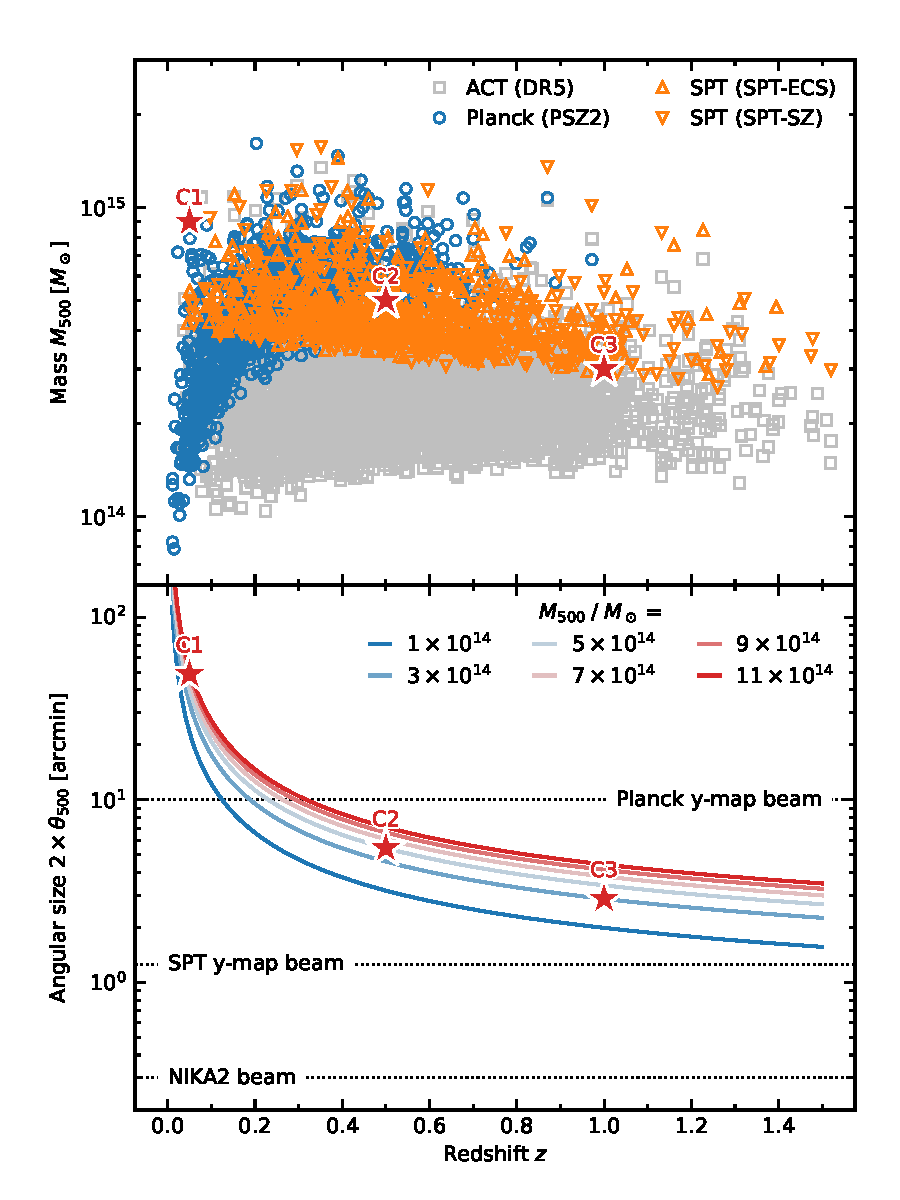
\includegraphics[width=\linewidth]{Figures/validation_sample.pdf}
    \caption{
        Validation cluster sample (black stars) in the mass-redshift plane (\textit{top panel}) and in the angular size-redshift plane (\textit{bottom panel}).
        For illustration, the top panel includes clusters detected in recent tSZ surveys: \textit{Planck} \citep{planck_collaboration_planck_2016-2}, ACT \citep{hilton_atacama_2021}, and SPT \citep{bleem_sptpol_2020,bleem_galaxy_2015}.
        Note that the redshift axis is truncated to $z<1.6$, therefore not showing all clusters in these samples.
        Colored lines in the bottom panel show the evolution of the angular $2\times\theta_{500}$ with redshift for clusters of different masses.
        The angular resolutions of the \textit{Planck} and SPT $y-$maps, as well as that of the NIKA2 camera at 150~GHz, are represented as dotted horizontal lines.
    }
    \label{fig:valid:sample}
\end{figure}

% -------------------------------------------------------------------------- %
\subsection{Data generation} \label{sec:simu:mkdata}

\begin{table*}[htp]
    \centering
    \begin{tabular}{l c c c c c}
        \toprule
        Instrument & Map size & Pixel size & FWHM & Filtering & White noise \\
        (Clusters) & $\theta_{\rm map}$ & $\theta_{\rm pix}$ & $\theta_{\rm FWHM}$ & & level \\
        \midrule
        \textit{Planck} & \multirow{2}{*}{$5\degree$} & \multirow{2}{*}{$2'$} & \multirow{2}{*}{$10'$} & \multirow{2}{*}{--} & Homogeneous \\
        (C1) & & & & & RMS=$4.12 \times 10^{-6} \; [y]$ \\
        \midrule
        SPT & \multirow{2}{*}{$30'$} & \multirow{2}{*}{$15''$} & \multirow{2}{*}{$1.25'$} & -- & Homogeneous, \\
        (C1, C2) & & & & & RMS=$9.78 \times 10^{-6} \; [y]$ \\
        \midrule
        NIKA2 & \multirow{2}{*}{$6.5'$} & \multirow{2}{*}{$3''$} & \multirow{2}{*}{$18''$} & NIKA2-like & Isotropic \\
        (C2, C3) & & & & transfer function & NIKA2-like RMS \\
        \bottomrule
    \end{tabular}
    \caption{\normalfont
        Properties of simulated maps emulating cutouts of the \textit{Planck} \citep{planck_collaboration_planck_2016} and SPT \citep{bleem_cmbksz_2022} $y-$maps, and NIKA2 cluster observations \citep{keruzore_exploiting_2020}.
    }
    \label{tab:simu:map_props}
\end{table*}

We create mock maps for the three clusters by forward modeling their tSZ signal.
We assume that each cluster has a pressure profile that follows the universal profile of \aten, scaled with its mass and redshift.
This pressure distribution is integrated along the line of sight to obtain a Compton$-y$ map.
This map is then projected on a flat-sky grid and convolved with a Gaussian filter to account for instrumental filtering, and added to a random noise realization.

As discussed previously, and illustrated in the bottom panel of figure~\ref{fig:valid:sample}, the angular size of each cluster is very different, and the mapping of their tSZ signal is very different for all instruments considered.
We therefore create different sets of maps for the three clusters.
For C1, the most extended cluster, we create mock \textit{Planck} and SPT maps.
For C2, our intermediate case, we create SPT and NIKA2 mock maps.
Finally, for C3, the smallest cluster in our sample, we only create mock NIKA2 data.
The characteristics of the maps are designed to mimic know cluster observations by the three instruments, and summarized in table~\ref{tab:simu:map_props}.
The generated maps are shown on the left panels of figure~\ref{fig:valid:dmr_2d}.

\paragraph{Planck-like data}  % ............................................ %
Our mock \textit{Planck} dataset is designed to emulate the \textit{Planck} \texttt{MILCA} Compton$-y$ map of \citet{planck_collaboration_planck_2016}.
The original data products for this map are in \texttt{healpix} format, which \panco\ cannot process, as it relies on the flat-sky approximation.
We therefore create maps of $(5\degree \times 5\degree)$ patches of the sky using a gnomonic projection, with a pixel size of $2'$, and a Gaussian PSF of ${\rm FWHM} = 10'$.
The noise in these maps is white and has an homogeneous distribution, with an RMS taken from the left panel of figure~13 in \citet{planck_collaboration_planck_2016}.
We do not consider any filtering of the signal aside from the beam convolution, as the scales filtered out by the data processing are very large compared to the size of the patch considered \citep[see][]{planck_collaboration_planck_2016}.

\paragraph{SPT-like data}  % ............................................... %
Our SPT-like maps mimic the publicly available $y-$map released by the SPT collaboration \citep{bleem_cmbksz_2022}, specifically the ``minimum variance'' map.
We use the same projection as their flat-sky maps, \ie\ a Sanson-Flamsteed projection with $15''$ pixels, on a $(30' \times 30')$ patch of the sky.
The resolution of the maps is Gaussian with ${\rm FWHM} = 1.25'$.
We inject white noise realizations, the amplitude of which is evaluated by computing the RMS of the map in a $(5\degree \times 5\degree)$ patch of the sky, taking care of masking sources.
The SPT $y-$maps use information from the \textit{Planck} $y-$map in the Fourier space to compensate for large-scale filtering, making it negligible ($<8\%$ filtering for angular scales $\ell < 2 \times 10^4$).
Therefore, we choose to consider no filtering in the creation of these maps.

\paragraph{NIKA2-like data}  % ............................................. %
Our NIKA2-like data imitates the NIKA2 150~GHz sky maps obtained by the NIKA2 SZ Large Program \citep{mayet_cluster_2020, perotto_nika2_2021}.
In particular, we use the data products publicly released in \citet{keruzore_exploiting_2020}.
We create a gnomonic projection of a $(6.5' \times 6.5')$ patch of the sky with $3''$ pixels.
The angular resolution of the map is Gaussian with ${\rm FWHM} = 18''$, and we also take into account filtering of angular scales due to data processing via the transfer function of \citet{keruzore_exploiting_2020}.
The noise in these NIKA2 maps is considered white and isotropic, but not homogeneous, as the NIKA2 on-the-fly scanning strategy used for obsevations of the NIKA2 SZ Large Program creates a variation in the noise level of the maps depending on the distance from the pointing coordinates.
To accurately take into account this effect, we use the noise RMS map of \citet{keruzore_exploiting_2020}, which we multiply by a scalar value to account for different exposure times.
Data produced by the NIKA2 collaboration is in NIKA2 150 GHz surface brightness units, usually presented in mJy/beam.
The conversion coefficient of $y-$to$-$mJy/beam can be evaluated by integrating the tSZ spectral distortion in the NIKA2 150 GHz effective bandpass (accounting for atmospheric opacity at the time of the observations), and is usually of the order of $-12$ mJy/beam/$y$ \citep[\eg][]{keruzore_exploiting_2020}, therefore we choose this value for our map generation.

% -------------------------------------------------------------------------- %
\subsection{Pressure profile fitting} \label{sec:simu:fit}

The five generated maps are then used to extract a pressure profile using \panco, \ie\ following the procedure detained in \S\ref{sec:algo}.
We assume that we know the characteristics of the map prior to fitting -- \ie\ the width of the beams used, the transfer function, and the noise RMS given to \panco\ in input are the same ones that have beed used to generate the maps.

Two ingredients in our model then remain to be specified: the radial binning -- \ie\ the value of the radii $R_i$ in eq.(~\ref{eq:algo:pressure_profile}) -- and the priors on the parameters.
For the radial binning, we choose one that is identically determined by the angular coverage of each map.
The first bin is defined as the projected radius corresponding to the size of a map pixel, $R_0 = \mathcal{D}_{\rm A}(z) \tan^{-1} \theta_{\rm pix}$, where $\mathcal{D}_{\rm A}(z)$ is the angular diameter distance to the cluster redshift $z$.
Four bins $\left\{R_1 \dots R_4 \right\}$ are then added, log-spaced between the projected sizes of the beam FWHM, $\mathcal{D}_{\rm A}(z) \tan^{-1} \theta_{\rm FWHM}$, and of the half map size, $\mathcal{D}_{\rm A}(z) \tan^{-1} \theta_{\rm map} / 2$.

The priors on each parameter is defined as follows.
For the pressure parameters $P_i$, corresponding to the value of the pressure profile at radii $R_i$, we compute the value of the universal pressure profile from \aten\ for the cluster's mass and redshift.
The prior on $P_i$ is then set as a log-uniform distribution around this value:
\begin{equation}
    \label{eq:simu:prior_Pi}
    p(P_i) = \log\mathcal{U}(10^{-2}, 10^2) \times P_{\rm A10}(R_i).
\end{equation}
The prior on the conversion coefficient is set as a Gaussian distribution.
For \textit{Planck}- and SPT-like maps, the data is directly in units of Compton$-y$, therefore this distribution is centered around 1.
For NIKA2 data, as discussed in \S\ref{sec:simu:mkdata}, the central value of the prior is set at $-12$ mJy/beam/$y$.
For all data, the spread of the distribution is taken as $5\%$ of its central value.

The MCMC sampling is run as presented in \S\ref{sec:algo:mcmc}, with $30$ walkers, and setting $n_{\rm auto} = 50$ and $\Delta\tau_{\rm max} = 5\%$.
For our tests, we used a 2021 MacBook Pro with an M1 Pro chip and a 10-core CPU, with the MCMC using 5 threads \todo{is this necessary?}.
With this setup and these criteria, each fit took 5 to 10 minutes to converge.
The raw Markov chains are then saved, and cleaned for the exploitation as described in \S\ref{sec:algo:outputs}, with $n_{\rm burn} = 500$, $n_{\rm discard} = 20$, and $q_{\rm extr} = 20\%$.

% -------------------------------------------------------------------------- %
\subsection{Results} \label{sec:simu:results}

The results of the regression is presented in Figures~\ref{fig:valid:dmr_2d} and \ref{fig:valid:profiles}.
Figure~\ref{fig:valid:dmr_2d} shows, for each of the five datasets, the simulated data (left), best-fitting 2D model (center), and the residuals (right).
The residuals panels show no significant structure, providing a visual indication of goodness of fit.
The right panels of Figure~\ref{fig:valid:profiles} also shows the data, model, and residuals, but as 1D azimuthal profiles, and include uncertainty computed from the spread of the sampled posterior.
The compatibility of the green curves (\ie\ residuals) with zero within uncertainties proves that \panco\ is able to retrieve a pressure profile that fits the data.

The left panels of Figure~\ref{fig:valid:profiles} show the pressure profiles recovered for each fit as the blue curves, including uncertainties.
The true profile used to generate each map data (\ie\ the universal \aten\ pressure profile for the cluster's mass and redshift, see \S\ref{sec:simu:mkdata}) is shown as a black dashed line.
For each data set, the agreement between the two curves across the considered radial range (\ie\ from the projected pixel size to the projected half map size) shows that \panco\ is able to retrieve an accurate estimation of the pressure profile of a cluster from its tSZ map.

\begin{figure*}[t]
    \centering
    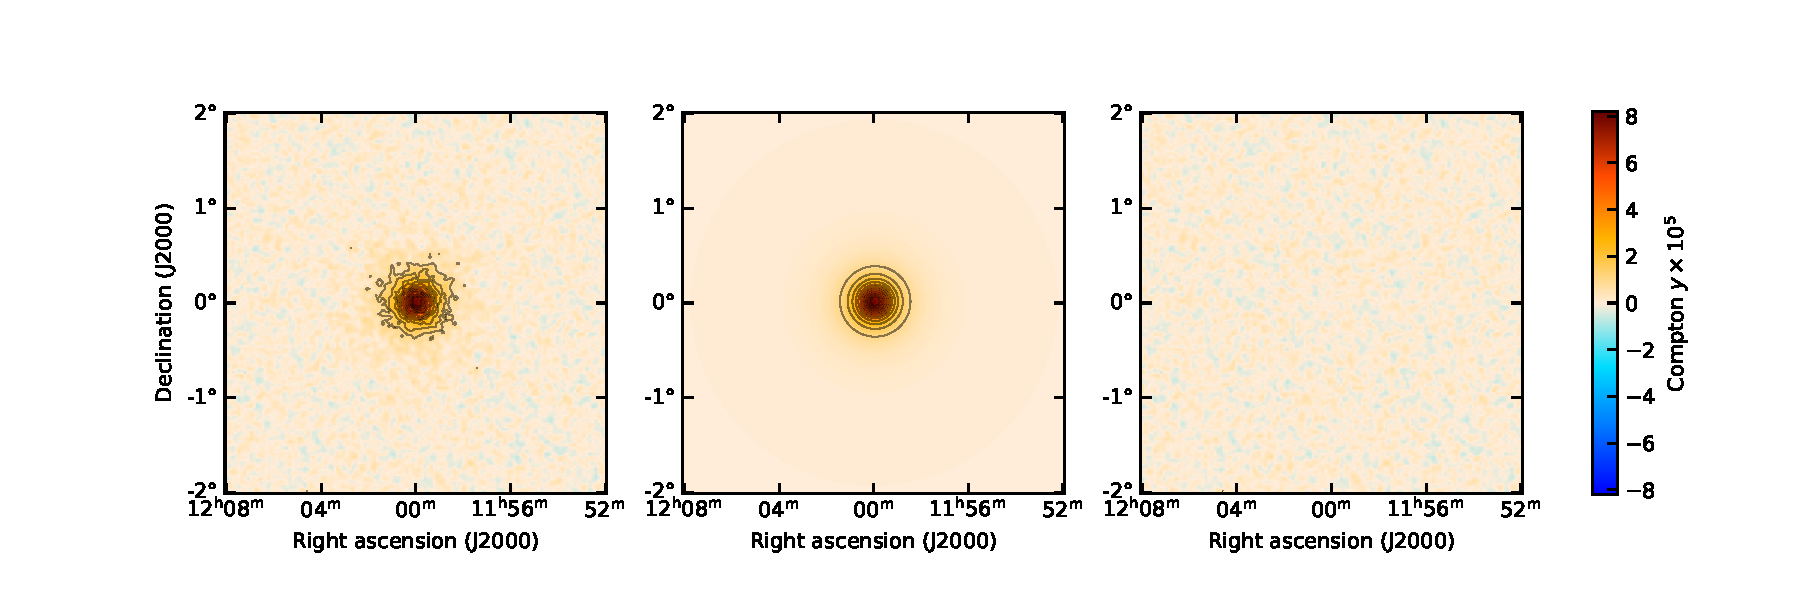
\includegraphics[height=4cm, trim={2cm 0.7cm 1.5cm 1.5cm}, clip]{../validation/results/C1/Planck/data_model_residuals_maps.pdf}
    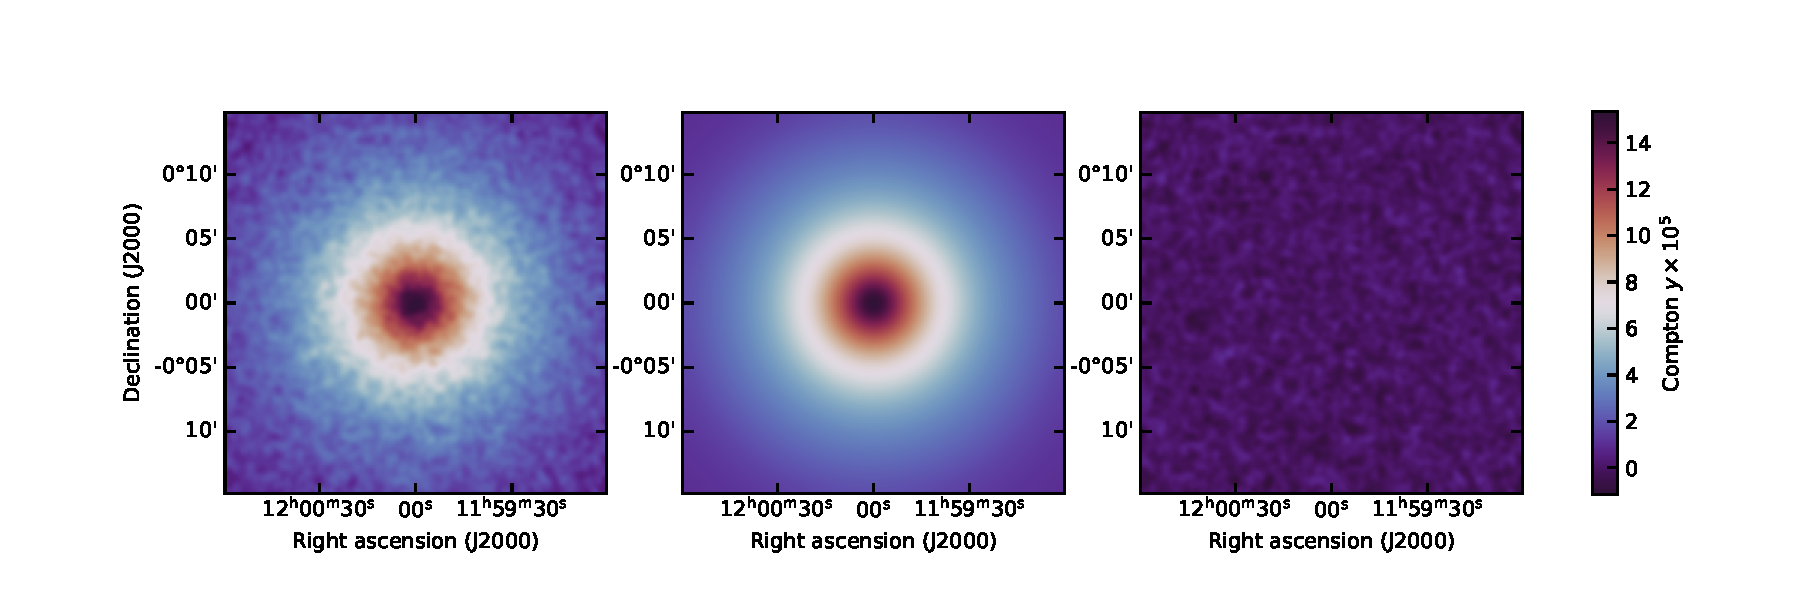
\includegraphics[height=4cm, trim={2cm 0.7cm 1.5cm 1.5cm}, clip]{../validation/results/C1/SPT/data_model_residuals_maps.pdf}
    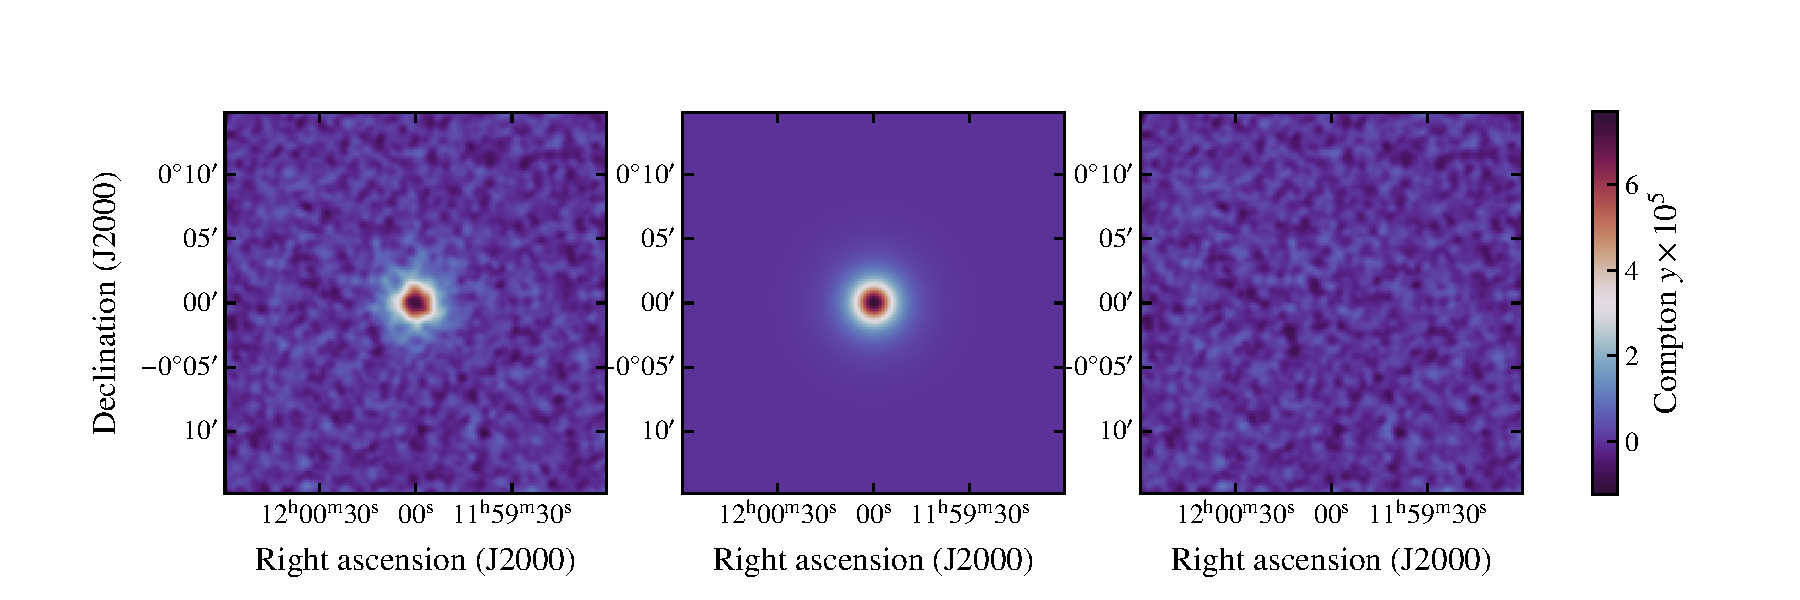
\includegraphics[height=4cm, trim={2cm 0.7cm 1.5cm 1.5cm}, clip]{../validation/results/C2/SPT/data_model_residuals_maps.pdf}
    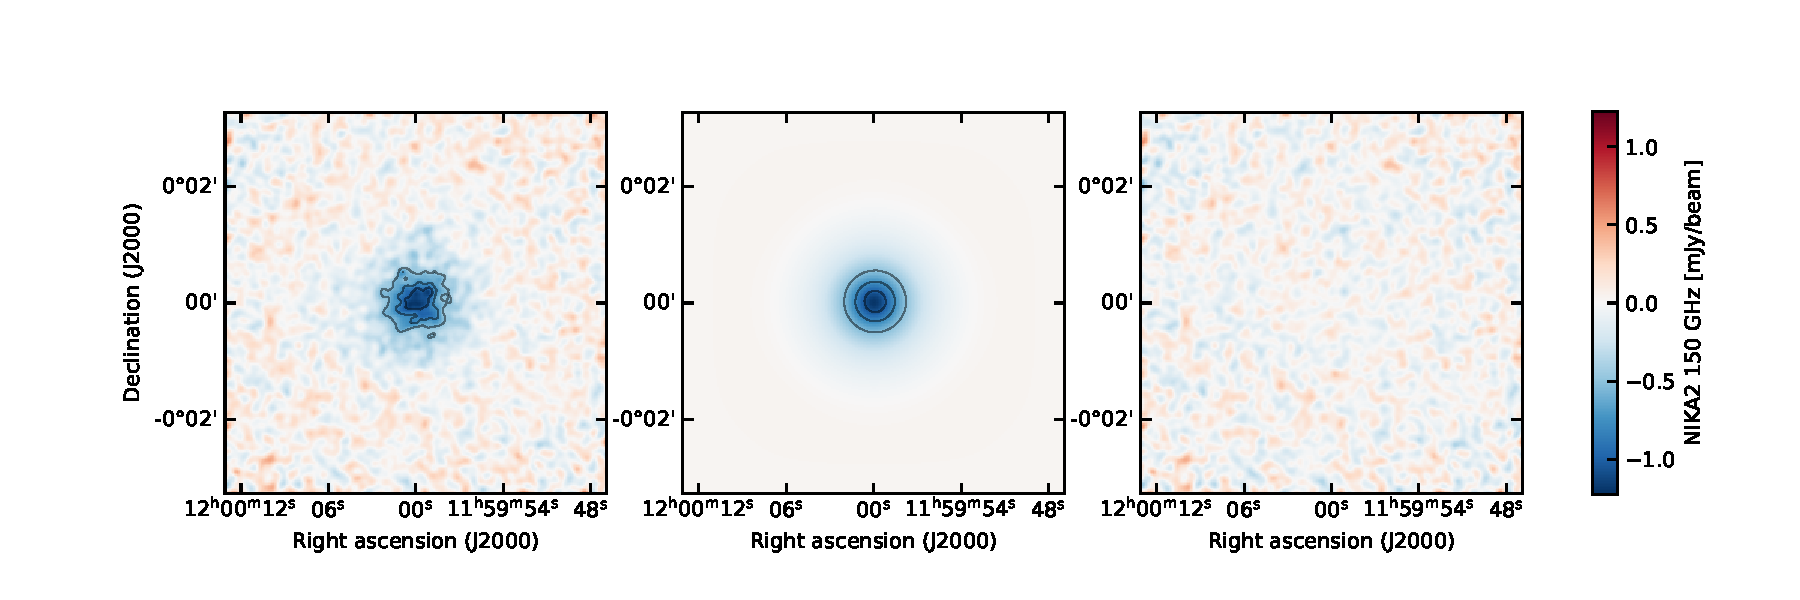
\includegraphics[height=4cm, trim={2cm 0.7cm 1.5cm 1.5cm}, clip]{../validation/results/C2/NIKA2/data_model_residuals_maps.pdf}
    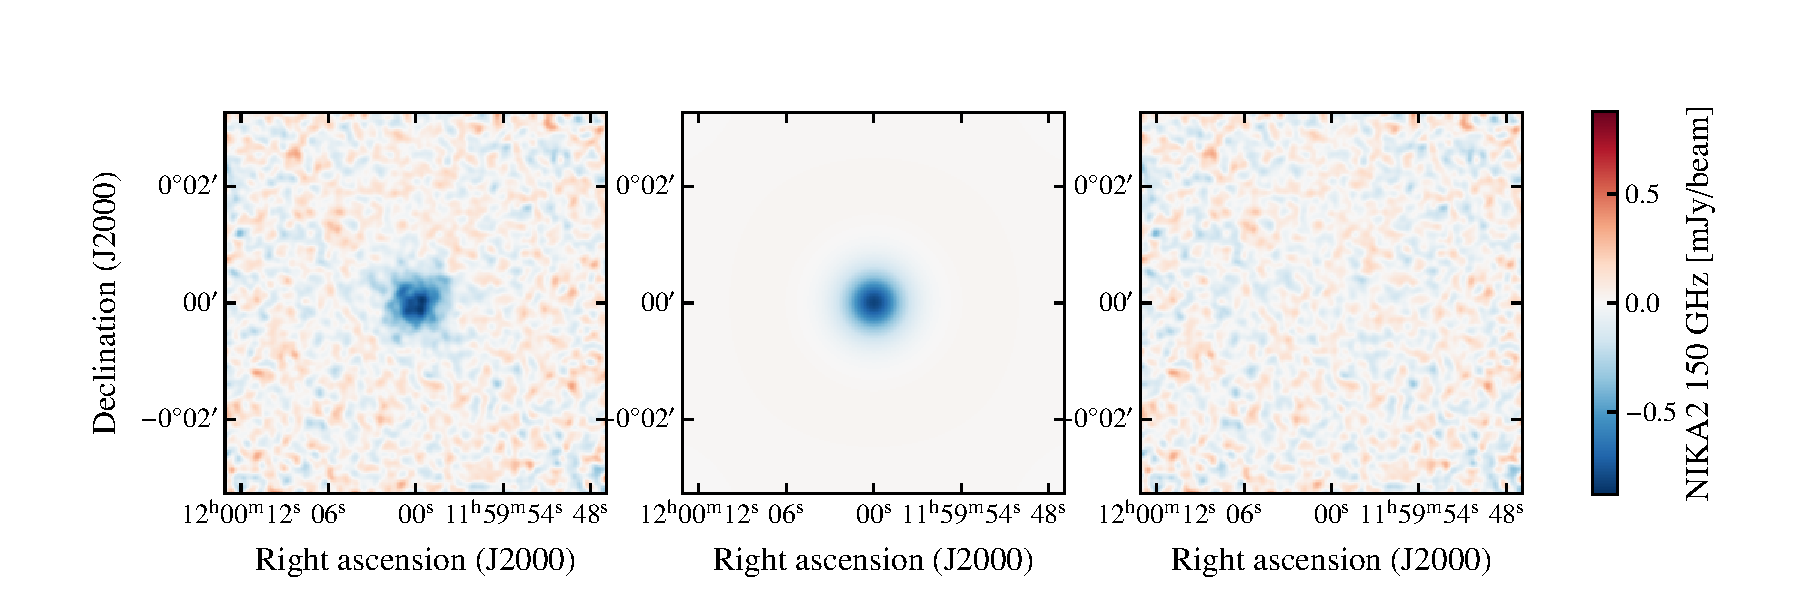
\includegraphics[height=4cm, trim={2cm 0.7cm 1.5cm 1.5cm}, clip]{../validation/results/C3/NIKA2/data_model_residuals_maps.pdf}
    \caption{
        Data (\textit{left}), model (\textit{center}), and residuals (\ie\ difference between data and model, \textit{right}) for the five validation fits:
        from top to bottom, C1 with \textit{Planck}, C1 with SPT, C2 with SPT, C2 with NIKA2, C3 with NIKA2.
        Maps are smoothed by a $1$ pixel Gaussian for display purposes.
        % Grey curves are signal-to-noise isocontours, starting at $3\sigma$ with a $2\sigma$ spacing.
    }
    \label{fig:valid:dmr_2d}
\end{figure*}


\begin{figure*}[t]
    \centering
    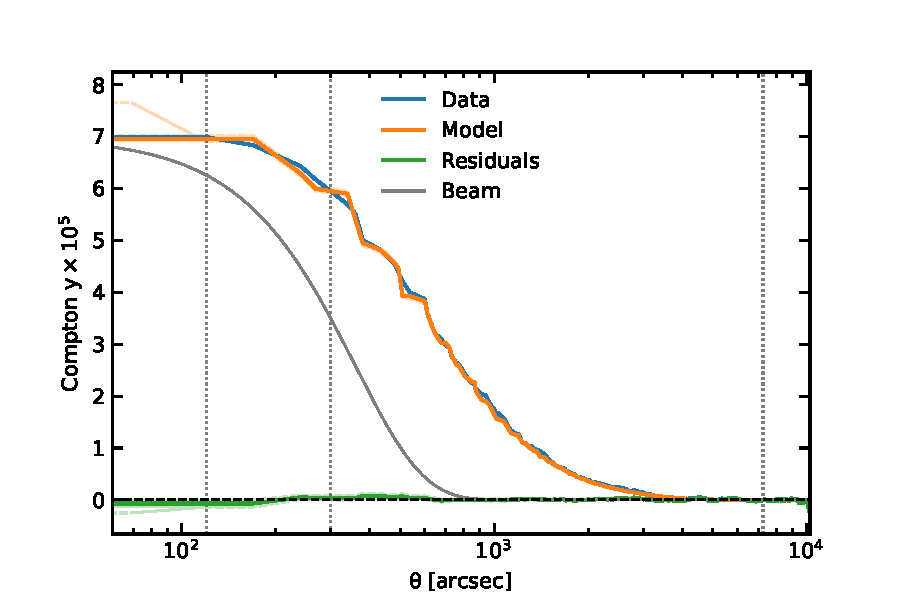
\includegraphics[height=4cm, trim={0 0 1cm 0.5cm}, clip]{../validation/results/C1/Planck/data_model_residuals_profiles.pdf}
    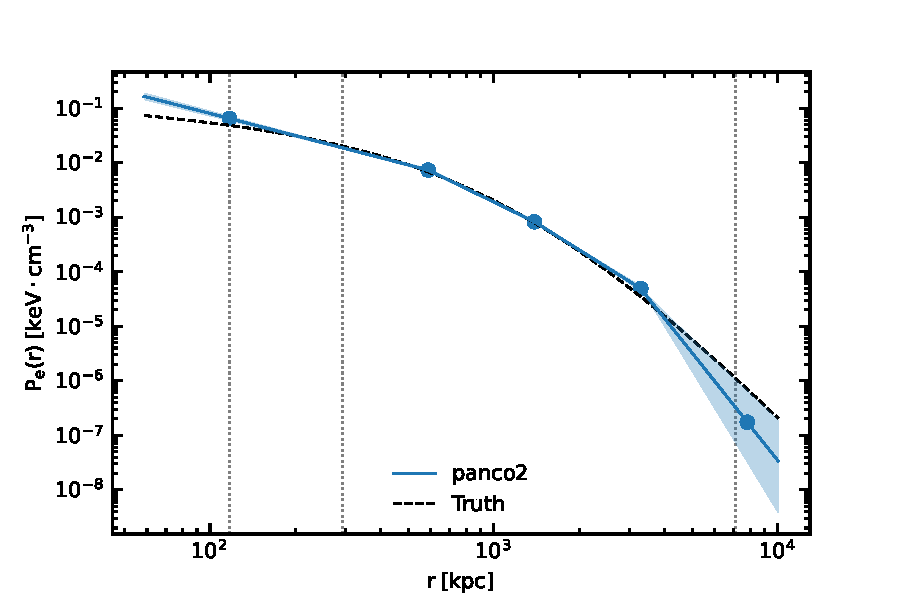
\includegraphics[height=4cm, trim={0 0 1cm 0.5cm}, clip]{../validation/results/C1/Planck/pressure_profile.pdf} \\
    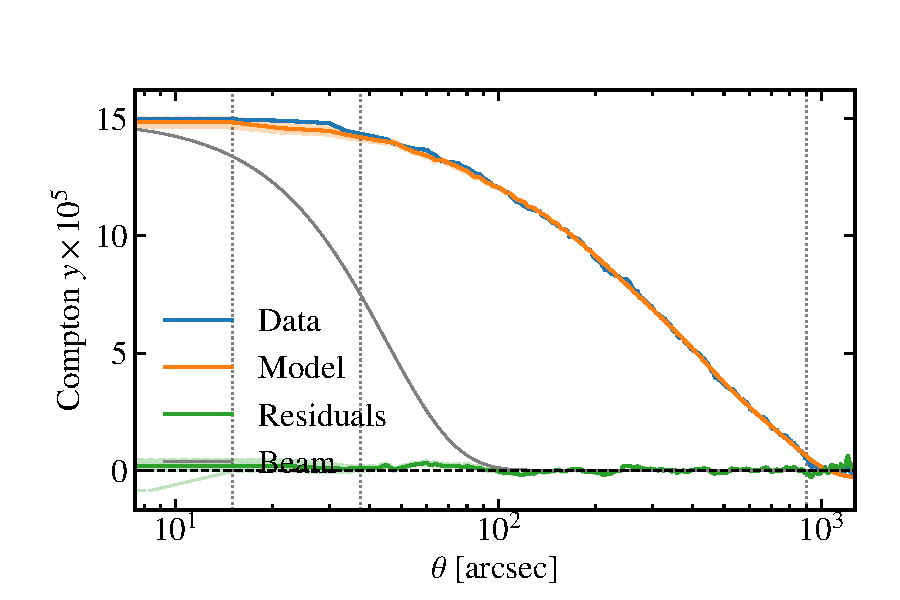
\includegraphics[height=4cm, trim={0 0 1cm 0.5cm}, clip]{../validation/results/C1/SPT/data_model_residuals_profiles.pdf}
    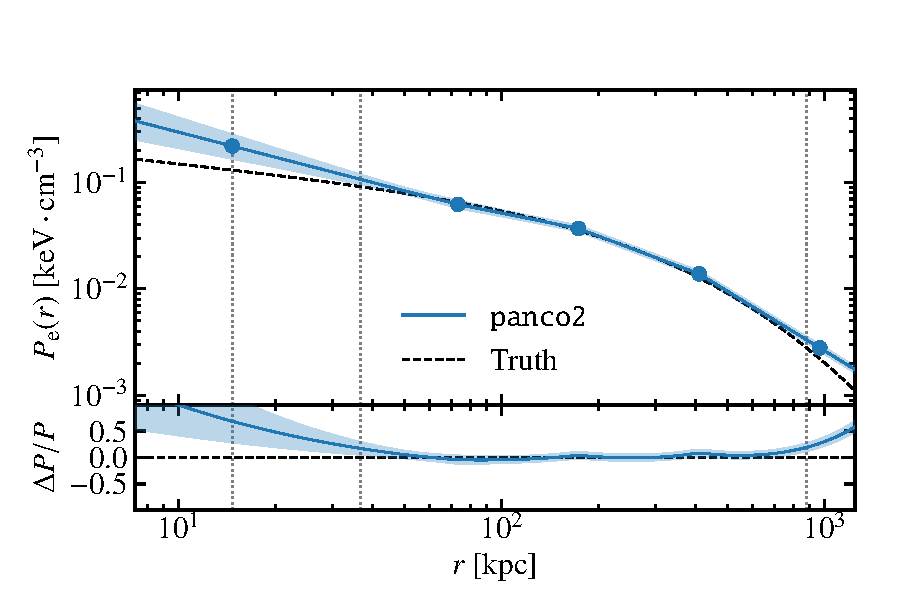
\includegraphics[height=4cm, trim={0 0 1cm 0.5cm}, clip]{../validation/results/C1/SPT/pressure_profile.pdf} \\
    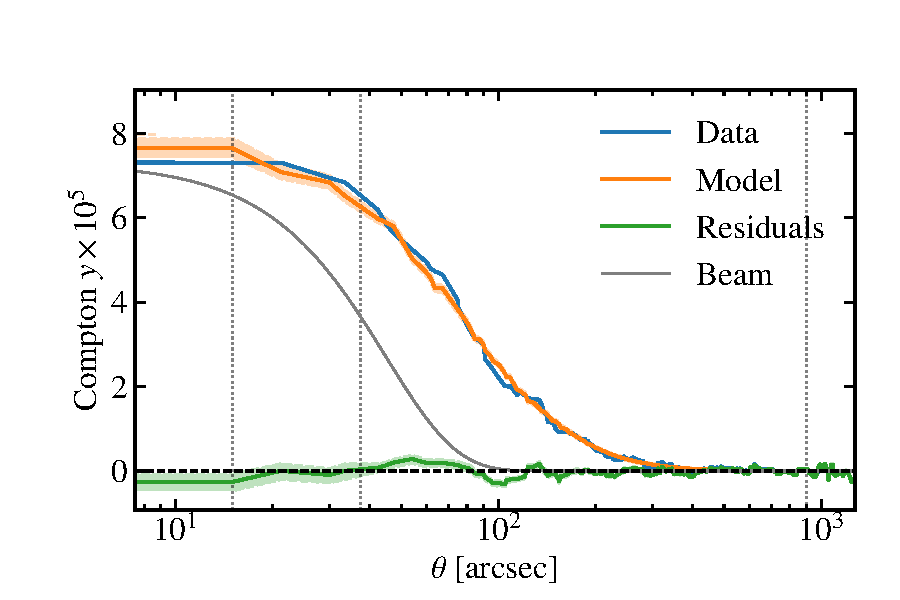
\includegraphics[height=4cm, trim={0 0 1cm 0.5cm}, clip]{../validation/results/C2/SPT/data_model_residuals_profiles.pdf}
    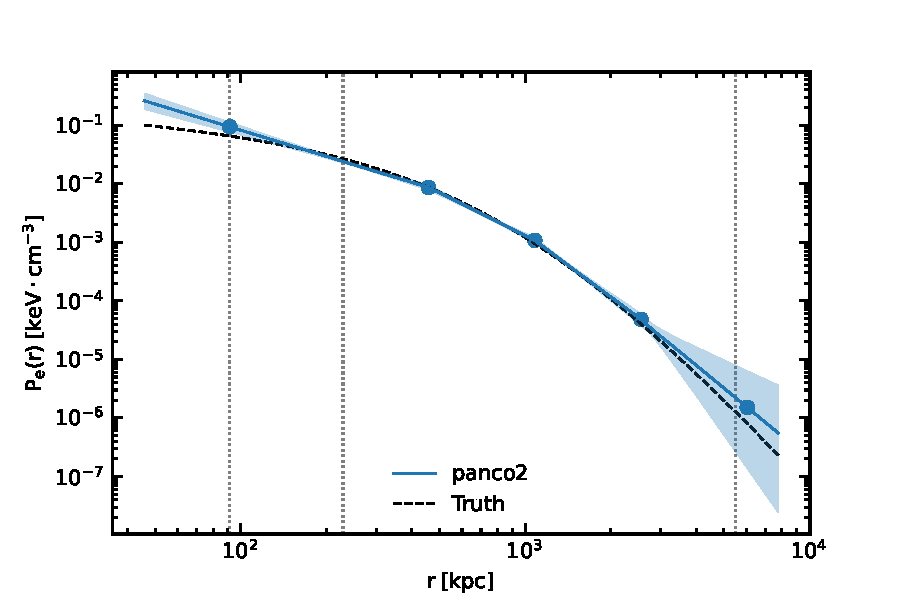
\includegraphics[height=4cm, trim={0 0 1cm 0.5cm}, clip]{../validation/results/C2/SPT/pressure_profile.pdf} \\
    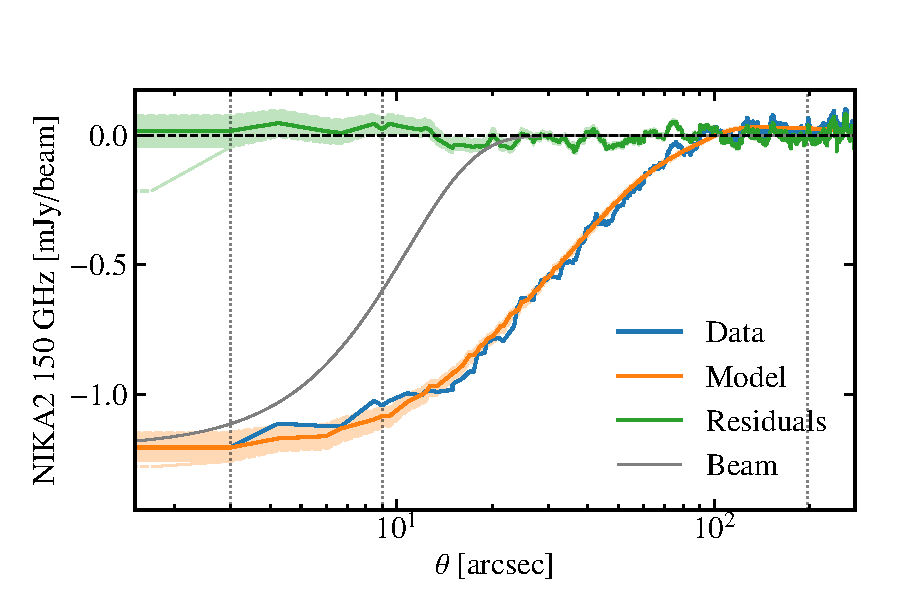
\includegraphics[height=4cm, trim={0 0 1cm 0.5cm}, clip]{../validation/results/C2/NIKA2/data_model_residuals_profiles.pdf}
    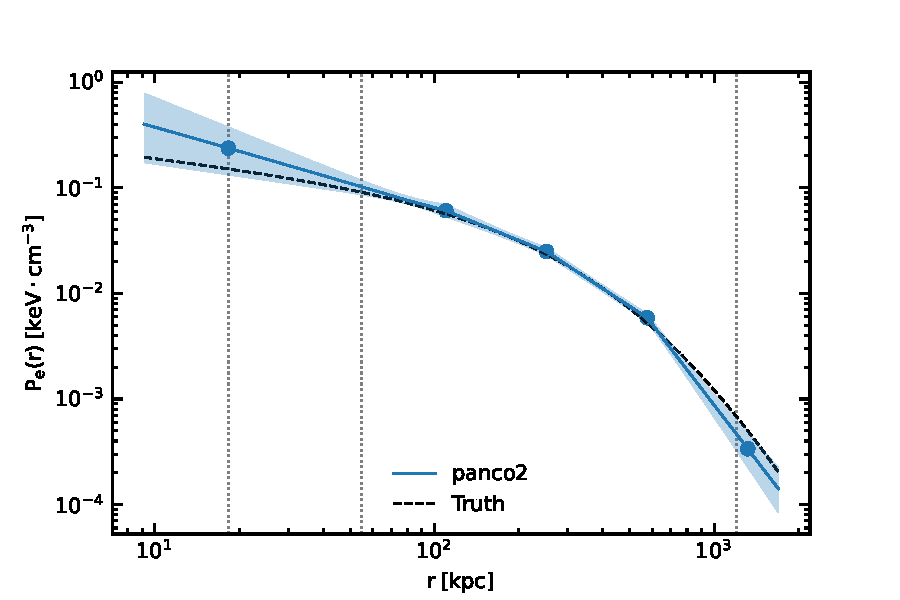
\includegraphics[height=4cm, trim={0 0 1cm 0.5cm}, clip]{../validation/results/C2/NIKA2/pressure_profile.pdf} \\
    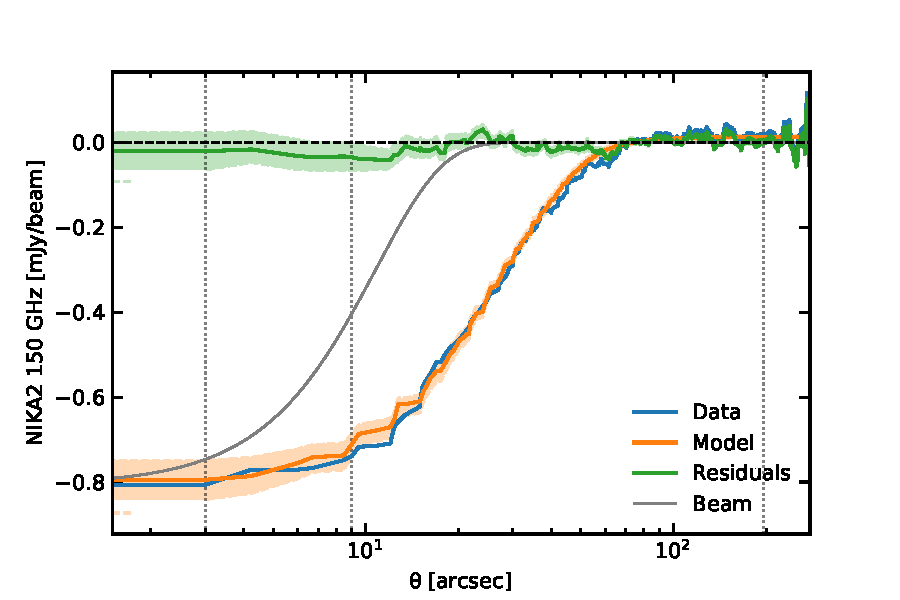
\includegraphics[height=4cm, trim={0 0 1cm 0.5cm}, clip]{../validation/results/C3/NIKA2/data_model_residuals_profiles.pdf}
    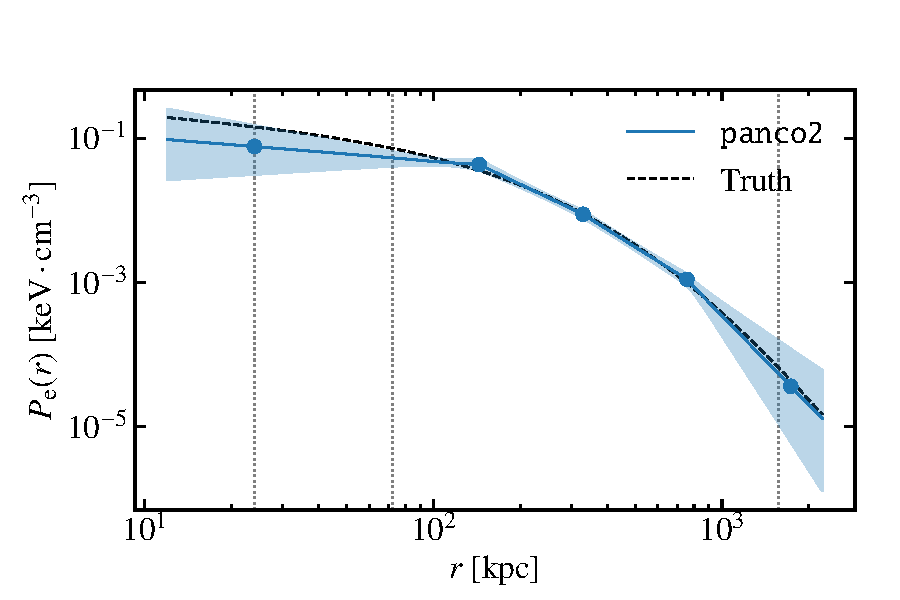
\includegraphics[height=4cm, trim={0 0 1cm 0.5cm}, clip]{../validation/results/C3/NIKA2/pressure_profile.pdf}
    \caption{
        \textbf{Left:} Data, model, and residuals (\ie\ difference between data and model) azimuthal profiles for the five validation fits.
        The beam profile is shown in grey for comparison.
        The rows are identical to Figure~\ref{fig:valid:dmr_2d}.
        \textbf{Right:} Pressure profiles reconstructed for each validation fit (blue line).
        For each profile, the shaded area marks the region between the 16th and 84th percentiles of the posterior distribution.
        The dashed black line shows the true pressure profile used to generate each map.
        In each plot, dotted vertical lines, from left to right, show the size of a map pixel, the beam HWHM, and the half map size.
    }
    \label{fig:valid:profiles}
\end{figure*}

% ========================================================================== %
\section{Conclusions and discussion}



\section*{Acknowledgements}
Thank you



%%%%%%%%%%%%%%%%%%%%%%%%%%%%%%%%%%%%%%%%%%%%%%%%%%
%%%%%%%%%%%%%%%%%%%% REFERENCES %%%%%%%%%%%%%%%%%%

\bibliographystyle{aasjournal}
\bibliography{panco2}

%%%%%%%%%%%%%%%%%%%% APPENDICES %%%%%%%%%%%%%%%%%%

\appendix

% !TEX root = ./main.tex
\section{some appendix}
\label{sec:app:1}

\textcolor{lightgray}{\lipsum[1]}


%%%%%%%%%%%%%%%%%%%%%%%%%%%%%%%%%%%%%%%%%%%%%%%%%%

% Don't change these lines
%\bsp	% typesetting comment
%\label{lastpage}
\end{document}
